\documentclass{article}
 
\usepackage[margin=1in]{geometry}
\usepackage[strict]{changepage}
\usepackage{float}
\usepackage{fancyhdr}
\usepackage{mhchem}
\usepackage{siunitx}
\usepackage{wrapfig, booktabs}
\usepackage{enumitem}
\usepackage{ctex}
\usepackage{graphicx}
\usepackage{amsmath}
\usepackage{amssymb}
\usepackage{subfigure}
\usepackage{multirow}
\usepackage{multicol}
\usepackage{wrapfig}
\usepackage{indentfirst}
\usepackage[utf8]{inputenc}
\usepackage{geometry}
\usepackage{setspace}   %set space between lines
\usepackage{graphicx} %insert figure 
\usepackage{float} %设置图片浮动位置的宏包
\usepackage{subfigure} %插入多图时用子图显示的宏包
\usepackage{listings}   %插入代码的宏包
\usepackage{xcolor} % to define color 
\usepackage{verbatim}   %for comment 
\usepackage[breaklinks,colorlinks,linkcolor=black,citecolor=black,urlcolor=black]{hyperref} %for bookmark 



\setlength{\parindent}{2em}

\definecolor{mygray}{rgb}{0.5,0.5,0.5}  %totally used in code display
\definecolor{mygreen}{rgb}{0,0.6,0}

\lstset{                %代码显示格式设置
    numbers=left,                                   
    % where to put the line-numbers; possible values are (none, left, right)
    numberstyle=  \color{mygray}, 
    % the style that is used for the line-numbers
    keywordstyle= \color{ blue!70},
    basicstyle=\footnotesize,        
    % the size of the fonts that are used for the code
    commentstyle=\color{mygreen},    
    % comment style
    frame=single,	                   
    % adds a frame around the code, you can use frame=shadowboxs
    % with a rulesepcolor= \color{ red!20!green!20!blue!20} ,
    escapeinside=``, % 英文分号中可写入中文
    xleftmargin=4em,xrightmargin=2em, aboveskip=1em,
    framexleftmargin=2em
} 


\begin{document}

\begin{spacing}{1.5}

    %title  page 
    \thispagestyle{empty}
    \begin{center}
~\\[6cm]\rule{\linewidth}{0.5mm} \\[6mm]
{\Large 综合论文  \\  \textbf{{\LARGE 心率传感电路}}  \\[6mm]}
\rule{\linewidth}{0.5mm} \\[2cm]
{\Large 姓 名: 吕光冉}\\[.3cm]
{\Large 班 级:   自73 }\\[.3cm]
{\Large 学 号:  2017011574}\\[.3cm]
{\Large 日 期:\today }\\[.3cm]
    \end{center}

    \clearpage
    \phantom{s}

    %if need to make table of contents in pdf, below command is okay
\tableofcontents
\newpage

    \subsection{摘要}

    本文介绍了一个基于光电测量法的心率测量电路的设计与实现。
    本电路设计以MK986脉搏心率传感器检测所得波形为输入信号,
    经过运放滤波和信号放大后,通过一个施密特比较器输出处理后的脉搏信号。
    同时,为了增强电路的可靠性,在面包板上搭建电路并验证工作状态无误后,
    我最终绘制了一块PCB板。在实验检测后。成功得到了比较理想的,符合数字
    电平的脉搏信号。

    \textbf{关键词} :心率测量电路,光电测量法,模拟电路设计

\section{引言——小米手环心率测量电路}

   我所选择的第一个综合论文题目为心率测量电路的设计与制作。

   之所以会选择这个题目,起源是我平时的一个小发现。
   有一次我在没有佩戴小米手环3的情况下,开启了其心率测量功能。结果我惊奇的发现,
   这时的小米手环测出了一个70多的数值。而当我再一次启动手环的测量功能后,
   我发现它竟然测出了180多的数值!
   
   对于我观察到的现象,一方面,我认为作为一款已经迈入市场的消费级电子产品,
   小米手环不应该在没人佩戴的前提下仍然能够测量到脉搏,这在我看来属于是产品设计缺陷。
   其次我认为,在所测量环境基本没有什么变化的时候,小米手环前后两次测量不应该有这么大
   差距。对这两个问题的好奇促使我去研究智能手环中心率测量电路的基本工作原理。
    
   经过调查发现,现在市面上存在的心率测量电路中,
   常见的测量原理有两种,一种是心动电流测量法,还有一种是光电透射(反射)测量法。

   第一种是心动电流测量法,需要使用到无线心率胸带。人体每次心脏跳动时,都会在胸口产生微弱的心动电流,
   而利用带有电极的无线心率胸带,就可以采集分析这样的电流,来对心率进行计数。
   这种测量方法的优点是测量十分精确,并且可以在运动过程中持续测量。但缺点在于其佩戴方式
   比较特殊,所以并不适用于普通消费者,而更适用于一些运动员。

   第二种是光电透射(或反射)测量法,这种测量方法也是智能手环测量心率的基本原理。
   光电透射测量法主要是利用了血液对光的吸收作用。由于在人体中,非血液成分对于光的吸
   收量基本是恒定的,而在血液中,静脉血的吸收波动相比于动脉血的吸收波动又十分微弱,可以忽略不计。
   所以,可以在恒定波长的光源照射下,通过监测“光的吸收率”这一模拟量的变化,并经过一定的滤波和计算后,
   就可以得到人体动脉血的跳动波形,从而获得心率跳动波形。

    其中,基于光电测量法的光电脉搏传感器通常又分成利用透射式和反射式两种。透射式的传感器
    其发射光源和光敏接收器件位于人体两侧,检测的是透射光光强变化,
    而反射式的传感器其光源和光敏器件位于同一侧,接收的是血液漫射和反射的光。
    由于智能手环本身的佩戴方式,其使用的是反射式的传感器。

   而本设计的设计目的为设计一个基于反射式光电透射原理的心率测量电路,最终要输出一个满足数字电平的
   脉搏信号,使得输出波形可以被后续 MCU 电路测量并进行数字处理。

\section{实现方案}

    我的心率测量电路设计方案如图\ref{fig:design_flow}所示:
    \begin{figure}[H]
        \centering
        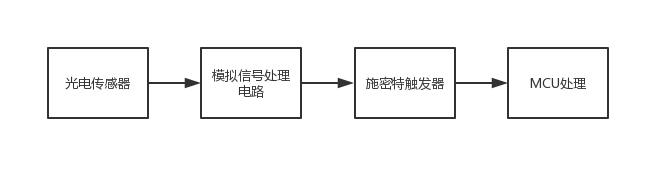
\includegraphics[scale=0.4]{fig/design/flow.png}
        \caption{整体设计方案}
        \label{fig:design_flow}
    \end{figure}
    
    在本设计中,光电传感器负责将血液跳动的光信号转化为微弱的电信号,然后经过模拟信号处理电路进行信号放大,噪声抑制以后,
    由施密特触发电路将模拟信号转化为可以由MCU处理的数字信号。

\section{电路原理分析}

    经过测量得知,第一级光电测量电路输出信号大致为一个有直流偏移的,变化幅值大致在100mV左右的脉搏波形。
    其中,直流电压会随着测量时间和接触的皮肤位置不同而变化,而脉搏波形的变化幅值也会因为传感器与皮肤接触的位置不同
    而变化。同时,传感器的输出电阻很小。    

    根据第一级光电传感器输出波形的以上特点,我设计的模拟信号处理电路原理图如图\ref{fig:design1}所示:

    \begin{figure}[H]
        \centering
        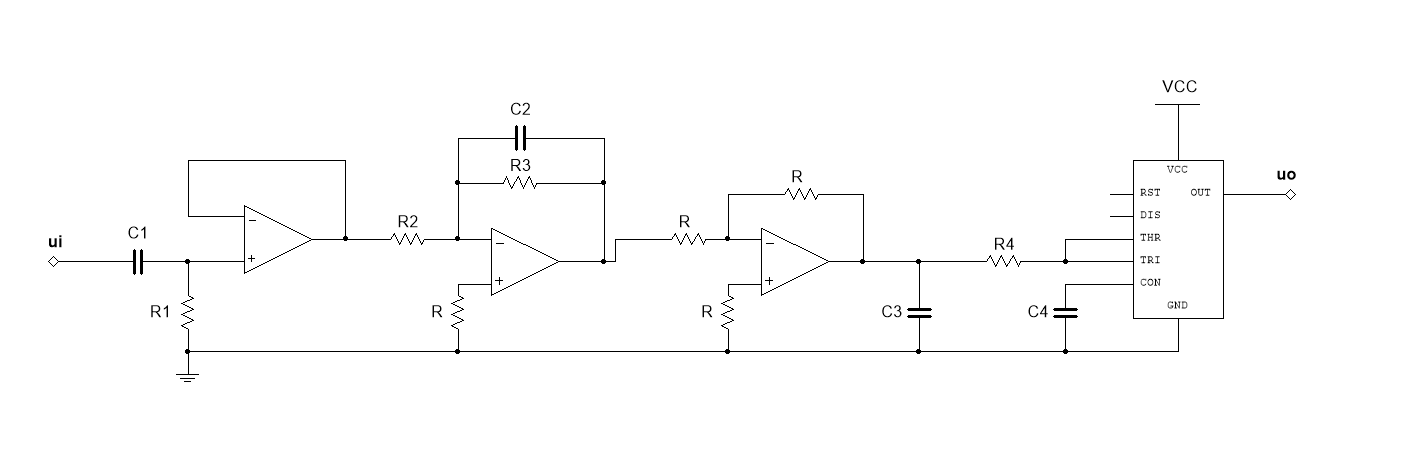
\includegraphics[scale=0.4]{fig/design/design1.png}
        \caption{模拟信号处理电路}
        \label{fig:design1}
    \end{figure}

    其中,第一级电路能隔离输入波形中的直流分量,并增大电路的输入电阻至$R_1$,
    第二级电路是一个微分器(相当于一个高通滤波器),并能够进行信号放大并进一步滤去低频噪声,
    第三级电路为低通RC电路和反相器,可以滤去输出级的高频噪声并将波形反向,
    最后一级电路为施密特触发器,可以将放大后的脉搏信号转变符合数字信号电平要求的脉搏信号。

    其中,对于中频段信号,模拟信号处理电路的输入输出电平之间的数学关系式为:
    \begin{equation}
        u_o = - \frac{R_3}{R_2} u_i
    \end{equation}

    通过表达式可知,在调试电路时,可以通过改变$\frac{R_3}{R_2}$ 来调整电路的放大倍数。

    而该电路的截止频率分别为:
    \begin{equation}
        \begin{cases}
            f_l = \frac{1}{2 \pi R_1 C_1}\\
            f_h \approx min \{ \frac{1}{2 \pi R_3 C_2}, \frac{1}{2 \pi R_1 C_1} \}
        \end{cases}
    \end{equation}

    所以可以通过调整 R1,C1,R3等参数来调整电路的幅频特性。

\section{整体电路仿真结果}

    我使用的仿真电路如图\ref{fig:sim1}所示。

    \begin{figure}[H]
        \centering
        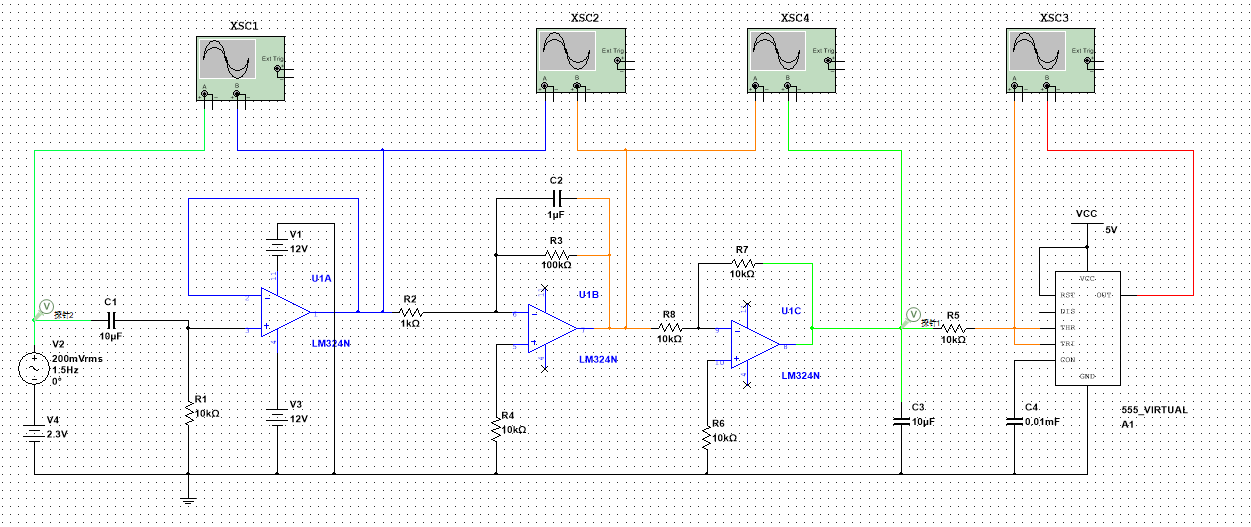
\includegraphics[scale=0.4]{fig/sim/sim1.png}
        \caption{心率测量电路仿真电路图}
        \label{fig:sim1}
    \end{figure}

    这里我用了一个直流电源和交流电源的叠加来模拟实际传感器输入信号。

    第一级电路的输入输出波形如图\ref{fig:sim1_result1}所示:
    \begin{figure}[H]
        \centering
        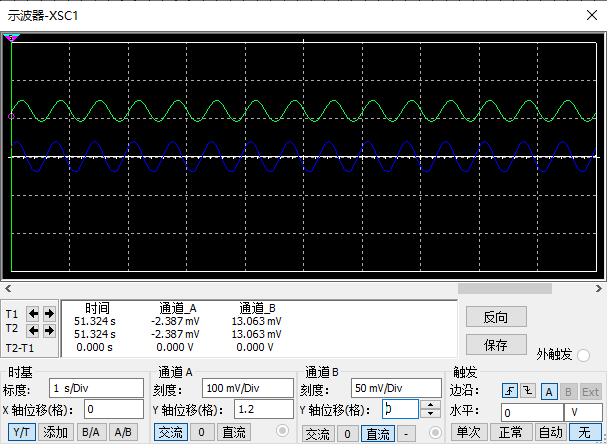
\includegraphics[scale=0.3]{fig/sim/sim1_result1.png}
        \caption{第一级电路传输特性}
        \label{fig:sim1_result1}
    \end{figure}
    
    从波形中可以看出,尽管有一定的相移,但是第一级电路已经成功滤去直流分量。

    第二级电路的电压传输特性如图\ref{fig:sim1_result2}所示:
    \begin{figure}[H]
        \centering
        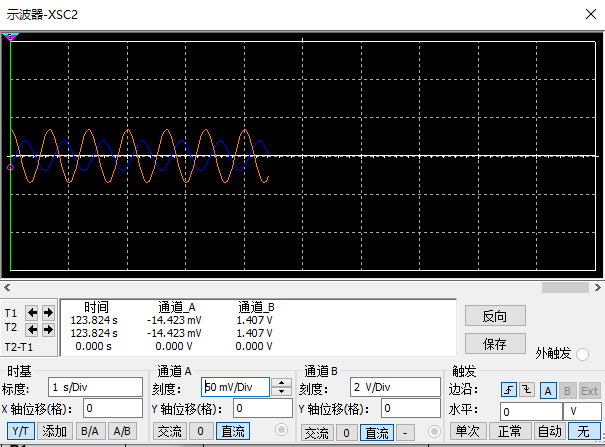
\includegraphics[scale=0.3]{fig/sim/sim1_result2.png}
        \caption{第二级电路传输特性}
        \label{fig:sim1_result2}
    \end{figure}
    
    此时,交流信号已经被成功放大。

    在经过低通滤波电路以后,施密特触发器的输入输出波形如图\ref{fig:sim1_result3}所示:
    \begin{figure}[H]
        \centering
        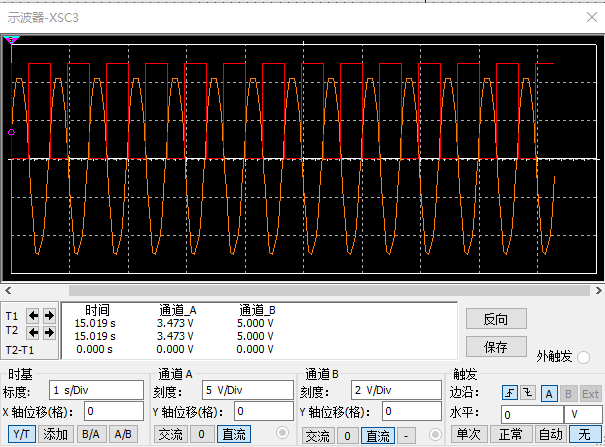
\includegraphics[scale=0.3]{fig/sim/sim1_result3.png}
        \caption{施密特电路输入输出波形}
        \label{fig:sim1_result3}
    \end{figure}
    
    可见,此时电路已经能够输出可以被MCU识别的数字信号。

    而对于模拟信号处理电路的幅频特性,仿真结果如图\ref{fig:sim1_result4}所示:
    \begin{figure}[H]
        \centering
        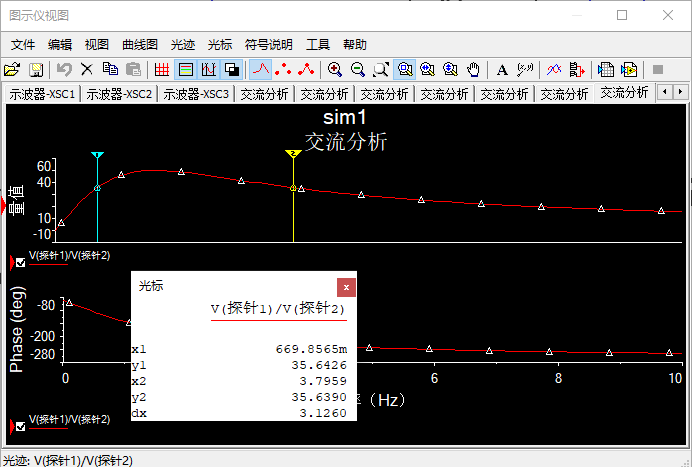
\includegraphics[scale=0.3]{fig/sim/sim1_result4.png}
        \caption{电路幅频特性}
        \label{fig:sim1_result4}
    \end{figure}

    可见,电路的低频截止频率为0.6Hz,高频截止频率为3.8Hz。这说明对于一般在1-3Hz的心跳信号,所设计的电路可以有效抑制
    电路高低频噪声并放大有效信号。

\section{电路搭建与实测结果}

    在面包板上搭建完电路并确认电路可以正常工作后,我在李兆基科技大楼绘制并现场制作了一块PCB板。
    但由于李兆基大楼的技术所限,
    我最终制作的仅仅是一块单面PCB板。制作成果如图\ref{fig:PCB1},\ref{fig:PCB2}所示:

    \begin{figure}[H]
        \centering
        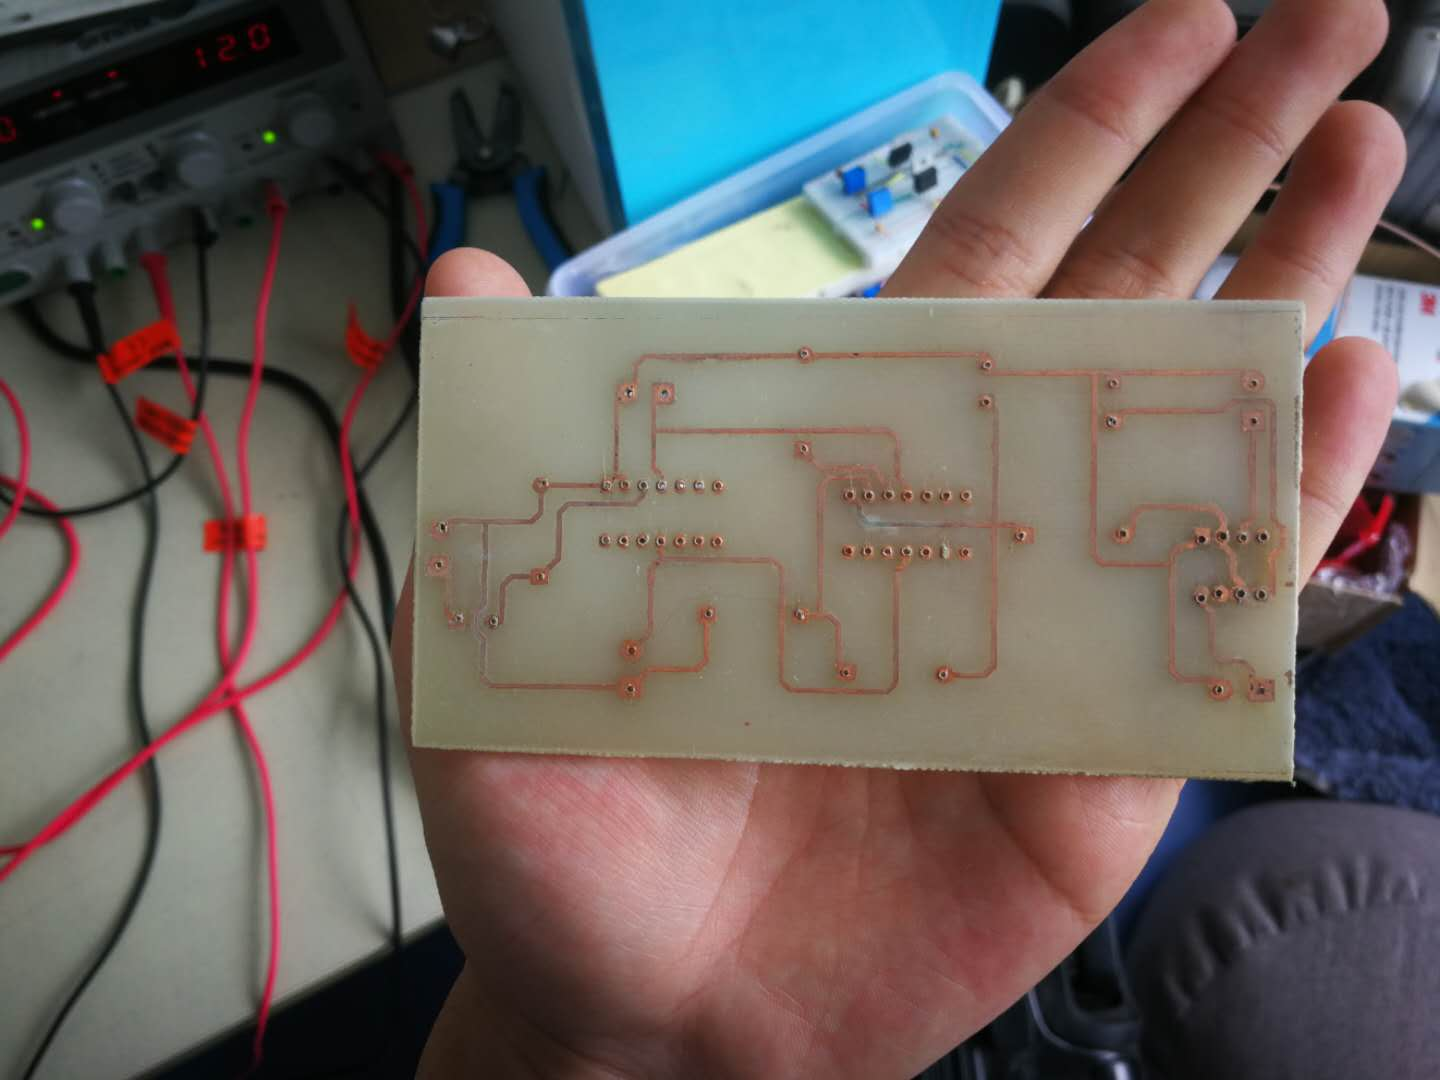
\includegraphics[scale=0.1]{fig/result/PCB1.png}
        \caption{PCB板-未焊接}
        \label{fig:PCB1}
    \end{figure}

    \begin{figure}[H]
        \centering
        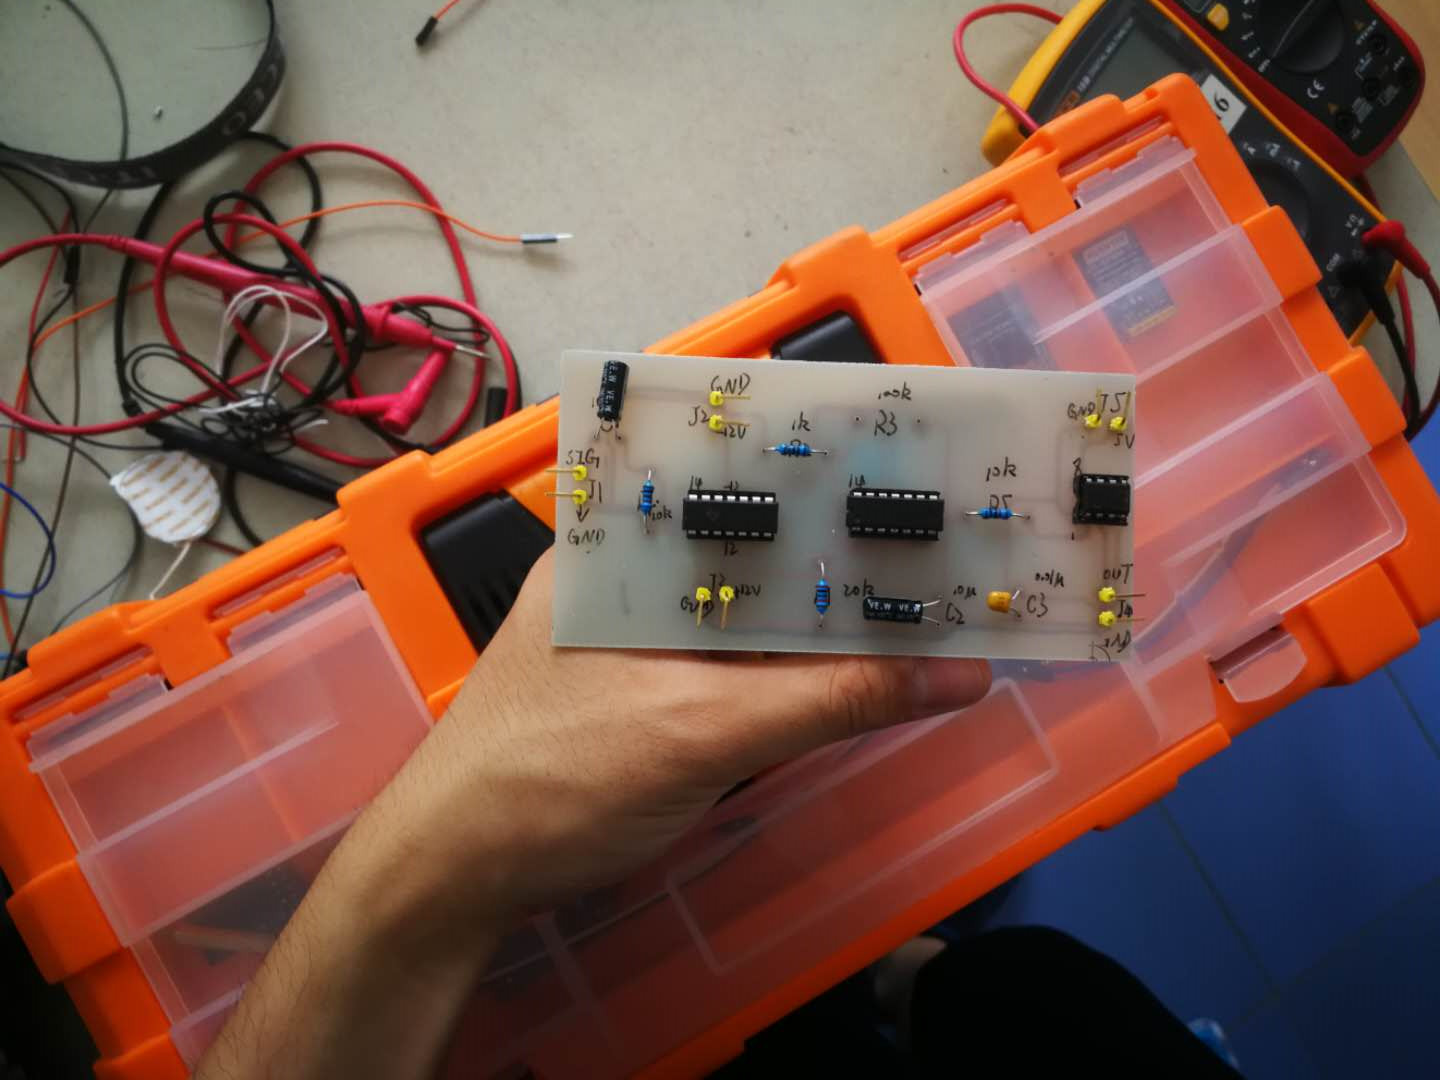
\includegraphics[scale=0.1]{fig/result/PCB2.png}
        \caption{PCB板-已焊接}
        \label{fig:PCB2}
    \end{figure}
    
    由于在绘制PCB板时,电路封装出现了一些问题,所以最后多使用了一块LM324芯片。

    之后我用魔术胶带将传感器绑在我的手腕上开始测量,如图\ref{fig:pulse1}所示:
    \begin{figure}[H]
        \centering
        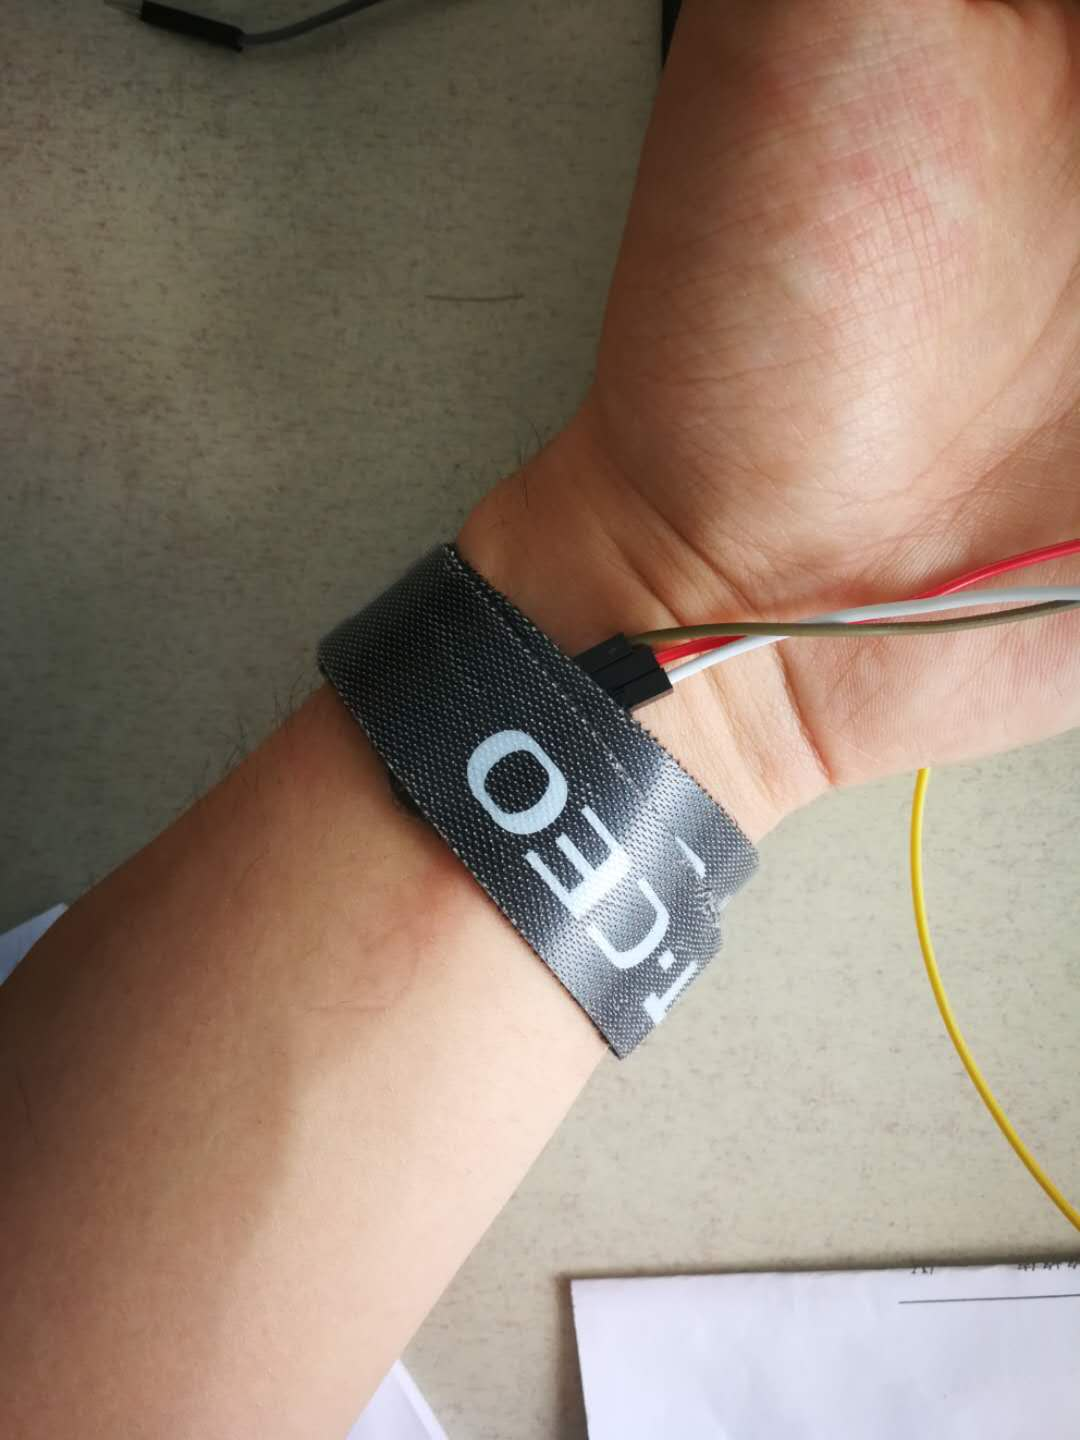
\includegraphics[scale=0.1]{fig/result/pulse1.png}
        \caption{传感器绑定方式}
        \label{fig:pulse1}
    \end{figure}
    
    此时,传感器输出波形如图\ref{fig:result1}所示:
    \begin{figure}[H]
        \centering
        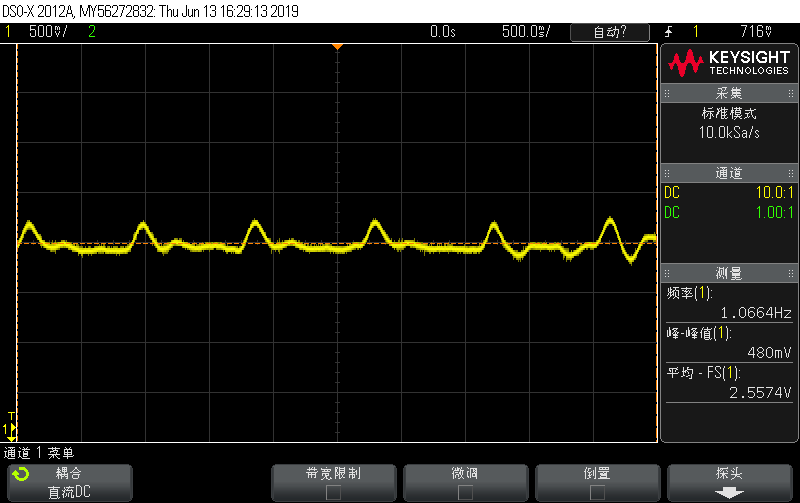
\includegraphics[scale=0.3]{fig/result/result1.png}
        \caption{传感器输出波形}
        \label{fig:result1}
    \end{figure}

    可见,此时传感器的输出波形中,存在一个2V以上的直流量。而有效的脉搏信号幅值大约有300mV,并且信号中存在
    高频噪声和中频(与脉搏信号频率相近的)噪声。
    
    第一级电路输出波形如图\ref{fig:result2}所示:
    \begin{figure}[H]
        \centering
        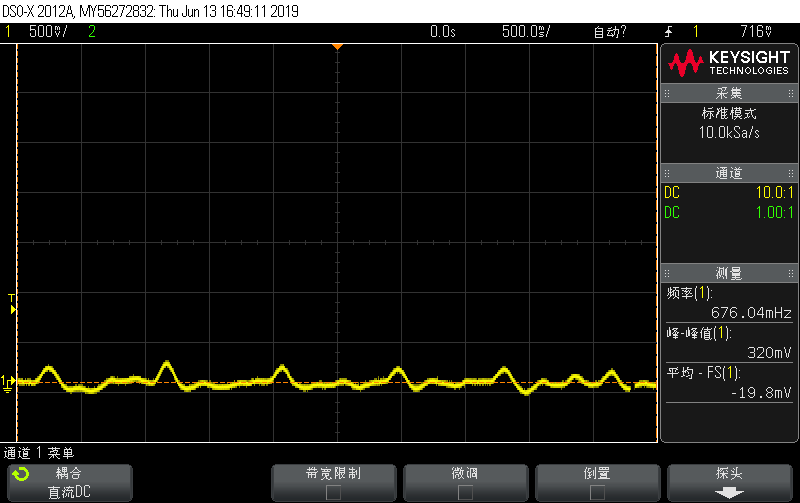
\includegraphics[scale=0.3]{fig/result/result2.png}
        \caption{第一级电路输出波形}
        \label{fig:result2}
    \end{figure}

    从输出波形可以看出,此时第一级电路已经成功滤去输入信号的直流分量。
    但同时,有效信号的幅值也被减少至200mV左右。

    第二级电路输出波形如图\ref{fig:result3}所示:
    \begin{figure}[H]
        \centering
        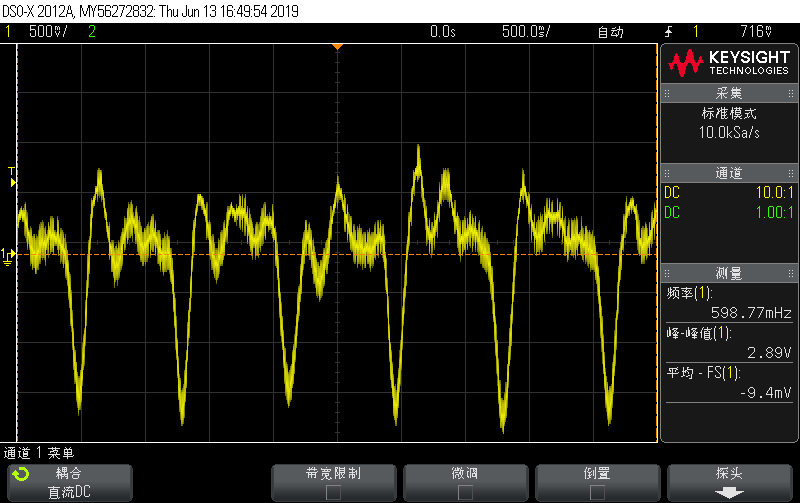
\includegraphics[scale=0.3]{fig/result/result3.png}
        \caption{第二级电路输出波形}
        \label{fig:result3}
    \end{figure}

    我在实际电路焊接时,我选择使用了一个100k可调电阻来代替仿真电路中的
    $R_3$ 电阻,这样就可以根据输入信号幅值的不同来手动调整电路放大倍数。
    
    如图\ref{fig:result3}所示的输出波形为调整放大倍数后的波形,
    可以看出,此时电路中与脉搏信号频率相近的干扰信号幅值不到1V,在反向后是无法触发施密特触发器的。
    这样一来就可以通过施密特触发器来过滤掉与脉搏信号频率相近的噪声。
    
    同时也可以观察到,在未进行高次噪声滤波前,电路中还是存在很强的高次噪声的。
    这样的噪声可以被后一级低通滤波器和施密特触发器抑制。但这也说明在下一版改进电路中,
    应该在前几级引入低通滤波器来提前抑制高频噪声。
    
    最后级电路输出波形如图\ref{fig:result4}所示:
    \begin{figure}[H]
        \centering
        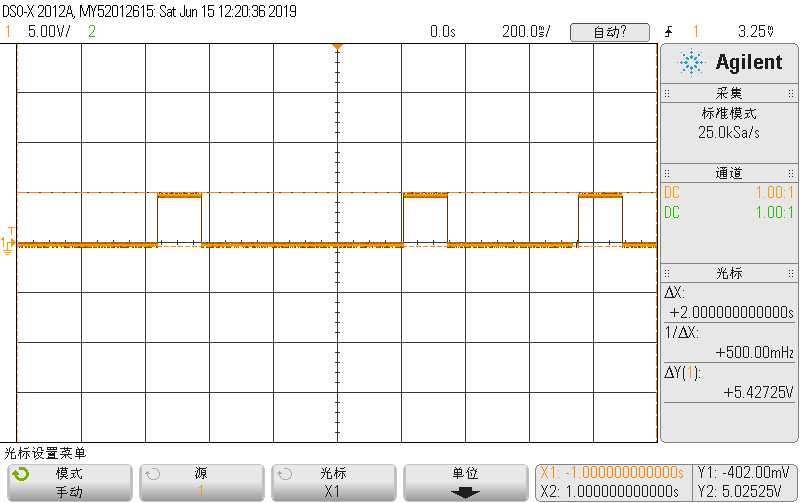
\includegraphics[scale=0.3]{fig/result/result4.png}
        \caption{第三级电路输出波形}
        \label{fig:result4}
    \end{figure}

    可以看出,这时电路已经获得了十分理想的,满足数字电平的脉搏波形。
    (这里的波形在第一次测量时忘记保存,图\ref{fig:result4}为后来补测的结果)。    

\section{实验中电路出现的问题以及原因分析}

    相对于我的第二个项目“智能风扇”,这个项目要简单许多。在制作过程中,我遇到的主要问题包括以下几点:

    \begin{enumerate}
        \item 忽略输出信号正负极性的问题
        
        为了在最后一级仅仅检测正极性信号,我才在最后一级选用了由555构成的施密特触发电路(不需要引入额外的参考电压),而不是
        使用在模电实验中我们通常使用的稳压管滞回比较器(需要引入额外的参考电压才能仅仅检测正电压)。 

        但是在第一次在面包板上搭建电路时,我忽略了第二级电路输出有反向的效果,这导致了原本想要检测的最为明显的
        正脉搏信号变成了负信号,无法被施密特触发器识别。

        这个问题在多引入了一个反相器后,得到了完美的解决。这也提醒我在电路设计时应该关注信号的极性问题。

        \item PCB绘制没有引出测试点
        
        由于是自己初次绘制PCB,没有足够的PCB绘制经验,所以在最终的电路中,PCB上引出的引脚
        只有各类电源和输入输出信号的引脚。
        这导致了在测试PCB电路工作状态时,由于焊接的元件引脚和示波器探头接触面积过小,
        探头上检测到的信号十分不稳定。
        
        所以说在PCB绘制时,应该事先考虑到测试的需要,在PCB板上引出合适的测试点以方便测试。

        \item 电源种类过多

        和我的第二个项目“智能风扇”相同的是,这个电路同样存在电源种类过多的问题。而电源种类过多一方面会增加电源管理模块
        设计的复杂度,另一方面会增大电路功耗,对于一款消费级电子产品是很不合适的。

        而根据所设计电路的实际工作状态,由于所处理的信号为变化的信号,所以电路是存在被改为单电源电路的可能性的。
        
        我初步设计的单电源脉搏检测电路如图\ref{fig:design2}所示:

        \begin{figure}[H]
            \centering
            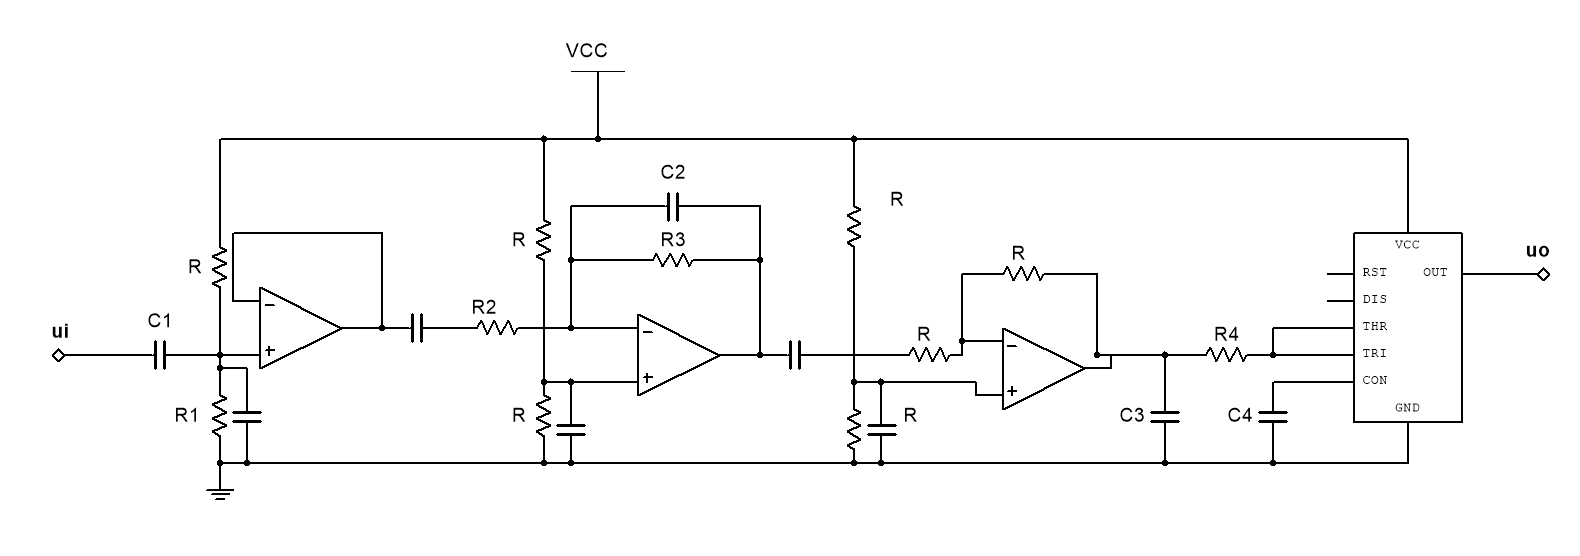
\includegraphics[scale=0.3]{fig/design/design2.png}
            \caption{第二版心率测量电路}
            \label{fig:design2}
        \end{figure}
        
        该设计中所有的LM324所接正电压为5V,负电压为0V。其中:
        \begin{enumerate}
            \item $R$ 和 $R_1$负责给运放提供2.5V的参考电位。
            \item $R_1$ 和 $C_1$ 构成高通滤波器,负责隔离电平直流量
            \item 第一级运放为跟随器,负责增大电路的输入电阻
            \item 跟随器后的电容起到进一步隔离直流分量的作用。
            \item R2,R3,C2和第二个运放构成反向微分器(相当于高通滤波器),同时起到放大信号的作用
            \item 第二级运放仍然设置其正极参考电位为2.5V
            \item 第三级运放为一个反相器,其基准电平仍然为2.5V
            \item R4,C3构成低通滤波器,负责过滤高频噪声。
            \item 最后一级由555构成施密特触发器,负责转化波形脉搏波形为数字信号波形。
        \end{enumerate}

        但是由于时间关系,我并没能完成这一版电路的仿真、实验和PCB绘制。这也是本项目的一个遗憾。

    \end{enumerate}

\section{项目的改进方向}

    项目的主要改进方向包括如下几点:

    \begin{enumerate}
        \item 提升传感器的稳定性。在实验时我发现,现在使用的脉搏测量模块工作状态并不完全稳定,其输出会因传感器所接触的皮肤位置不同
        而产生明显变化,
        以致于略微移动一下传感器的位置,就会出现脉搏信号检测不到的问题。
        所以在后续电路改进时,应该首先考虑更换传感器来提升电路工作的稳定性。

        \item 减少电源数量。在最终搭建的电路中,所使用的电源种类过多,包括有正负12V,正5V三种电源。一方面,种类过多给
        电路的搭建和调试带来很大的不便,另一方面,如果该心率传感电路要被融入到消费类电子产品中,减少电源数量可以
        有效的降低因电平转换而消耗的功率,从而提升便携式电子设备的电路工作时间。

        \item 在前几级电路中引入一定的低通滤波器以滤出高频噪声。在实际测量过程中,我发现电路中存在很多的高频噪声,这
        一点在第一版电路设计的时候是没有考虑到的。

    \end{enumerate}

\end{spacing}
\end{document}